%%%%%%%%%%%%%%%%%%%%%%%%%%%%%%%%%%%%%%%%%%%%%%%%%%%%%%%%%%%%%%%%%%%%%%%%%%%%%%%%
%2345678901234567890123456789012345678901234567890123456789012345678901234567890
%        1         2         3         4         5         6         7         8

\documentclass[letterpaper, 10 pt, conference]{ieeeconf}  % Comment this line out
                                                          % if you need a4paper
%\documentclass[a4paper, 10pt, conference]{ieeeconf}      % Use this line for a4
                                                          % paper

\IEEEoverridecommandlockouts                              % This command is only
                                                          % needed if you want to
                                                          % use the \thanks command
\overrideIEEEmargins
% See the \addtolength command later in the file to balance the column lengths
% on the last page of the document

\usepackage[utf8]{inputenc}
\usepackage[T1]{fontenc}
\usepackage{listings}
\usepackage{xcolor}
\usepackage{listings}
\usepackage{graphicx}
\usepackage{xparse}
\usepackage{threeparttable}
\usepackage{array}
\usepackage{tabularx}
\usepackage{subcaption}
\usepackage{tablefootnote}

\newcolumntype{Y}{>{\centering\arraybackslash}X}
\newcolumntype{L}{>{\raggedleft\arraybackslash}p{.2in}}
\newcolumntype{R}{>{\raggedright\arraybackslash}p{.2in}}
\NewDocumentCommand{\codeword}{v}{%
\texttt{\textcolor{black}{#1}}%
}

\lstset{language=C,keywordstyle={\bfseries \color{blue}}}

% The following packages can be found on http:\\www.ctan.org
%\usepackage{graphics} % for pdf, bitmapped graphics files
%\usepackage{epsfig} % for postscript graphics files
%\usepackage{mathptmx} % assumes new font selection scheme installed
%\usepackage{mathptmx} % assumes new font selection scheme installed
%\usepackage{amsmath} % assumes amsmath package installed
%\usepackage{amssymb}  % assumes amsmath package installed
\usepackage{hyperref}
\usepackage{multicol}
\title{\LARGE
\textbf{Price Prediction with Neural Networks:\\ Time Series Forecast meets Deep Learning}\\
\Large
CSC 240 Final Project
}

%\author{ \parbox{3 in}{\centering Huibert Kwakernaak*
%         \thanks{*Use the $\backslash$thanks command to put information here}\\
%         Faculty of Electrical Engineering, Mathematics and Computer Science\\
%         University of Twente\\
%         7500 AE Enschede, The Netherlands\\
%         {\tt\small h.kwakernaak@autsubmit.com}}
%         \hspace*{ 0.5 in}
%         \parbox{3 in}{ \centering Pradeep Misra**
%         \thanks{**The footnote marks may be inserted manually}\\
%        Department of Electrical Engineering \\
%         Wright State University\\
%         Dayton, OH 45435, USA\\
%         {\tt\small pmisra@cs.wright.edu}}
%}
\author{Minh Khoi Nguyen Do, Vuong Ho, Chuqin Wu, Qianwen Fu}


\begin{document}



\maketitle
\thispagestyle{empty}
\pagestyle{empty}


%%%%%%%%%%%%%%%%%%%%%%%%%%%%%%%%%%%%%%%%%%%%%%%%%%%%%%%%%%%%%%%%%%%%%%%%%%%%%%%%
\begin{abstract}
    For the final project of CSC240, we look to apply deep learning techniques in the subject of time series analysis and analyze their performance in this type of task, and possibly compare their accuracy against autoregressive methods, which are algorithms specially developed for time series data. Specifically, we look at whether neural networks can be applied in the financial sectors by using a variety of networks such as bidirectional RNN, GRU, and LSTM to predict future prices of Microsoft stocks, Bitcoin, and similar datasets with varying levels of features. We have also prepared and generated artificial time series datasets that simulate reality to see how deep learning can be applied in this kind of task. We find that all four of the networks we experimented with perform relatively well on our datasets and that some networks perform better at one dataset than the other. 

\end{abstract}


%%%%%%%%%%%%%%%%%%%%%%%%%%%%%%%%%%%%%%%%%%%%%%%%%%%%%%%%%%%%%%%%%%%%%%%%%%%%%%%%
\section{INTRODUCTION}
\subsection{About time series}
    Oxford Languages defines "time series" to be "a series of values of a quantity obtained at successive times, often with equal intervals between them" \cite{oxford}, and in mathematics, a time series is "a series of data points indexed (or listed or graphed) in time order" \cite{enwiki:1057905873}. Definition asides, time-series data appears in every part of our life. From every day's temperature and rain level on the East Coast of the United States, to the stock price of AAPL or Ethereum fluctuating every time the market opens, each and every one of us has seen and directly experienced this type of data. Interested in this simple-sounding yet difficult to understand, for our final project we decide to analyze time series, and specifically, time series prediction.

\subsection{Time series prediction and analysis}
    People have always wanted to see and predict the future. Looking at a chart of time series data, it is inevitable that each one of us has wondered at least once about what tomorrow will be like. How will the data behave? Will it go up, or will it go down? Having the ability to predict the future would be great! We would be able to know about what tomorrow's temperature will be during our picnic trip, or whether this cryptocurrency that we have invested our entire life savings in will make us appear in the next Forbes 30 under 30, or will it just pull us deeper in the red. However, accurately predicting the future is an impossible thing to do, but with the power of mathematics, we can at least make an educated guess.
            
    Predicting the future is not just for getting rich quick in the stock market; but rather, time series prediction can help researchers in the medical field predict the number of traumas of each person \cite{nademi}, or hospitals in Southern Taiwan to forecast emergency visits \cite{Juange018628}, or farmers in Idukki district, Kerala to predict rainfalls \cite{kamath2018}. Due to its varying use in all fields, the subject of time series forecasting is widely researched, all the way back in the latter half of the 20th century, with many algorithms having been developed, and widely used, for this kind of task, most notably autoregressive methods.

\subsection{Deep learning in time series forecasting}
    With autoregressive methods seeming to be the go-to algorithms for this task, our team decides to take a step back and approach this problem in a different way: using deep learning. Consider that the task of time series prediction is taking an input of time series data and output future price, this is the perfect task for a neural network to train on and perform predictions based on the trend learned from the training process. We noticed a specific type of neural network with structures very suitable for the tasks of learning from long series of data: recurrent neural network (RNN). With the context of one state being included in the next state of the training process, we think that this would allow the RNN to pick up on historical trends, and from that give a good educated guess.

    With that said, we are interested in seeing the performance of RNN and its variants in the price prediction task in financial datasets, the extent to which some techniques can be used and their effectiveness, and how well they work in both real-life time-series datasets and artificial ones. Specifically, we are comparing the performance of four different RNNs structures, namely traditional RNN, bidirectional RNN, GRU, and LSTM on 6 datasets, 4 real-world datasets including Microsoft stock price at market close, S\&P500 Index, crude oil prices, and Bitcoin price, and 2 artificially generated datasets.

\section{Literature Review}
    The application of deep learning into the time series prediction is not novel: Brownlee (2018) details on how to construct a deep learning network for this purpose using a wide variety of techniques including Multilayer Perceptrons, Convolutional Neural Networks, and Recurrent Neural Network to predict many different types of datasets \cite{brownlee2018}, Gamboa (2017) explores similar approaches to time series dataset with deep learning \cite{gamboa2017deep}, Qiu et al. (2014) proposes a deep learning belief network for regression and time series forecasting and also experiments with support vector regression \cite{7015739}. Deep learning in financial datasets has even been explored for over a decade, way back in 2005 by finance researchers in both the academic world and the industry \cite{SEZER2020106181}, and many others in different fields, such as healthcare (Miotto et al. (2017) \cite{10.1093/bib/bbx044}, Kaushik et al. (2020) \cite{10.3389/fdata.2020.00004}, Purushotham et al. (2018) \cite{PURUSHOTHAM2018112}), agriculture (Guillén-Navarro et al. (2020) \cite{navarro2020}, Jin et al. (2020) \cite{s20051334}, Atef et al. (2021) \cite{9531929}), weather (Salman et al. (2015) \cite{7415154}, Hossain et al. (2015) \cite{7280812})...

    Individually, there have also been many papers looking at the performance of each of the variants of RNN.
    \subsubsection{Long-Short Term Memory (LSTM)}
        Althelaya et al. (2018) utilizes a bidirectional LSTM structure (a bidirectional LSTM being a two-way LSTM with information from hidden states taken in from both the previous and the future states) to perform prediction on the S\&P 500 Index and finds that this structure performs well on the applied datasets, with final loss of 0.03247 with MAE (Mean Absolute Error) loss and 0.04211 with RMSE (Root-mean-square Deviation) loss \cite{8355458}. 

    \subsubsection{Gated Recurrent Unit (GRU)}
        In research from Shen et al. (2018), a 3-layer GRU model with an input layer of 240 timesteps and 25 hidden neurons has been implemented for multi-class classification \cite{SHEN2018895}. Its performance on the S\&P 500 Index achieved an accuracy of 51.4\%. The author confirmed that it is effective to use GRU to extract useful information from financial time-series data. Similarly, Dutta et al. implemented a simple GRU with 50 hidden neurons and one dense layer with one hidden neuron on the same Bitcoin price dataset \cite{dutta2019}. The size of the input layer depending on the lookback ranged from 15 to 60 days. The regression achieved an RMSE of 0.01 on the training set and 0.019 on the testing set. Therefore, these two studies proved that GRU is a valid method for learning and predicting non-linear patterns in complex financial data. In addition, as Dey et al. (2021) pointed out in their comparative analysis of RNN in stock price prediction, besides outperforming the simple RNN, GRU even produced a better loss than LSTM especially when the lookback period gets shorter \cite{a14080251}.

\section{Methodology}
    In time series dataset, any piece of data at any given point in time may depend on the data before and after it, which means that context matters a lot in determining a value in time. Due to this property of time series data, recurrent neural networks seem to be best fit for this job, and so we will be applying this type of networks along with their variations for our analysis. Specifically, we will be using in total four recurrent-type neural networks which are: 
    \begin{itemize}
        \item Traditional RNN
        \item Bidirectional RNN
        \item Gated Recurrent Unit (GRU)
        \item Long-Short Term Memory (LSTM)
    \end{itemize}
    which we will apply on a variety of financial datasets and compare their performance in each of the datasets. The following sections detail our reason for choosing these 4 methods.
    
    \subsection{Why RNN?}
        Recurrent Neural Networks (RNNs) are a class of neural networks that “are naturally suited to processing time-series data and other sequential data” (DiPietro \& Hager, 2020 \cite{zhou_rueckert_fichtinger_2020}). Traditional RNN is the base model of the other RNN variants. Its basic structure is shown in the diagram:
        
        \begin{figure}[thpb]
            \centering
             \includegraphics[width=5cm]{image/11.png}
            \caption{Structure of an RNN cell (Soleimany, 2020) \cite{soleimany}.}
            \label{figurelabel}
        \end{figure}

        \begin{figure}[thpb]
            \centering
             \includegraphics[width=8cm]{image/12.png}
            \caption{Hidden state formula in an RNN cell (Li, Johnson \& Yeung, 2017) \cite{li_johnson_yeung}.}
            \label{figurelabel}
        \end{figure}

        It takes into a sequential input vector, does calculations for the hidden units, and then gives an output vector based on the calculations. The hidden units are the key to enable processing sequential data since the current hidden state is calculated based on the input vector and the previous state. This dependency memorizes the historical data and preserves the order of the sequential data. A sigmoid function is used in hidden states calculations in order to introduce non-linearity to our model as real-life data is usually non-linear. The weight matrix is found by finding gradients during the backpropagation process to minimize the loss function of choice. The same function and set of parameters will be used for calculating all the hidden states as shown in the equation diagram.

    \subsection{Bidirectional RNN}
        Bidirectional RNN, as its name suggests, is a recurrent neural network whose information flows both ways during the training process. First introduced in 1997 in the paper by Schuster and Paliwal (1997), bidirectional RNN is a direct extension of the original recurrent neural network, with the ability to learn from both past and future contexts due to its two-way nature. As noted by the authors, the structure of the bidirectional RNN contains two sets of state neurons of a traditional RNN that are responsible for either forward and backward states. Inputs are fed to both context flow, but outputs from forward are not given to inputs of backward states, and vice versa. (see figure below)
        
        \begin{figure}[thpb]
            \centering
             \includegraphics[width=8cm]{image/13.png}
            \caption{Structure of a BRNN model (Schuster, 1997).}
            \label{figurelabel}
        \end{figure}

        The authors remarked that since the network is considering both past and future information, it allows the objective function to be directly minimized "without the need for delays to include future information", in contrast to the regular unidirectional RNN. Experiments with bidirectional RNN confirms its better performance than the regular RNN in some cases (Cao et al. (2018) propose BRITS (Bidirectional Recurrent Imputation for Time Series), a slight modification of bidirectional RNN, with an 11.56 MAE loss, lower than the 14.24 of RNN), and we speculate that the bidirectional RNN would work better in our time series prediction tasks than the traditional RNN, as well, due to its ability to pick up more context (from both future and past).

    \subsection{Gated Recurrent Unit (GRU)}
        GRU is a gating mechanism developed from RNN by Cho et al. in 2014. Every hidden state contains two gates: the forget gate decides how much information in the past hidden state to forget and the update decides how much past information to retain. As shown in the equation, gates are calculated through the sigmoid function to have an output ranging from 0 to 1. Thus, we can consider the output from the gate as a percentage of information from the past hidden states. The gating mechanism addresses the problem of vanishing gradients in traditional RNN by storing the information of past states in the two gates, and it also has less computational complexity than LSTM.

        $$ z_t = \sigma(W_z \cdot [h_{t-1},x_t])$$
        $$ r_t = \sigma(W_r \cdot [h_{t-1},x_t])$$
        $$ h_t = (1-z_t) \ast h_{t-1} + z_t \ast \tilde{h}_t$$
        $$ \tilde h_t = tanh(W \cdot [r_t \ast h_{t-1}, x_t]_j)$$

    \subsection{Long-Short Term Memory (LSTM)}
        The idea of LSTM is developed by Sepp et al. in 1997. Here, we refer to the use of modern paper to explain the mechanism of LSTM. The LSTM has one additional element compared with the hidden state and it is the cell memory, so it could store both long-term and short-term information. There are three gates in the LSTM cells. They are input, forget, and output gates. The input gate decides how to handle the hidden state from the previous cell and the input of the current cell. The output gate decides how to forward the information of the cell to the next cell. The forget gate decides which information the cell could ignore and place more emphasis on more important ones. 

\section{Network Implementation}
    \subsection{Traditional RNN}
        We implemented a 1-layer traditional RNN model with 64 hidden neurons on the six datasets by using PyTorch packages. The inputs are grouped in batches to facilitate the backpropagation process. For datasets with large numbers of samples - artificial 1, bitcoin, and artificial 2 datasets - we group them into 64 batches, while for Microsoft stock, crude oil, and S\&P 500 stock datasets, we use 32 batches. To improve the robustness of our model and prevent overfitting, we used a dropout rate of 0.2 and the RELU activation function to train our model. Moreover, we did 50 epochs on the S\&P 500 stock dataset and 20 epochs on the other datasets since the S\&P 500 dataset needed more epochs to converge during backpropagation. 

    \subsection{Bidirectional RNN}
        The structure of the bidirectional RNN is very similar to the above traditional RNN, but with the RNN cell replaced with bidirectional RNN cells. We also apply some changes in the internal linear output layers to take in double the hidden output size, since the output of the bidirectional RNN is doubled in size compared to the RNN. The internal bidirectional RNN cell contains 64 hidden layers. This neural network trains on 50 epochs for all datasets at a learning rate of 0.001, with an input batch size of 32 or 64 based on sample size, and a lookback of 5 days, or time steps. 

    \subsection{GRU}
        A one-layer GRU was implemented with an input size equal to the lookback of 5 days and 64 hidden neurons in one hidden state. One dense layer of linear function followed it to output the final prediction. Using the TensorDataset and DataLoader method from Pytorch, we transformed the data to tensors and separated them with different batch sizes 32 or 64 based on the sample size. With a learning rate of 0.001, the model was run separately using different loss functions for backpropagation to check the consistency of the prediction results.

    \subsection{LSTM}
        We develop the LSTM model by Pytorch. We use the first LSTM layer with the purpose of mapping input features to the first hidden features. Then we connect that to the second LSTM layer to map to the second hidden feature. Then, we connect every feature at the end through a dense layer to output the next number of steps we want. We also initialize hidden states to zero to begin the training then keep propagating the hidden states to later training batches. With a learning rate of 0.001, the model was run separately using different loss functions for backpropagation to check the consistency of the prediction results. We output the loss of train and test set through the number of epochs to see the general trend in training. We also plot the predicted values to compare with the test values to visualize that. We apply training, testing, and plotting for every dataset.

    \subsection{Loss Metric}
        We used two different loss functions, MSE and L1 (MAE), to do backpropagation and recorded the losses separately to compare the performances. Doing so, we believe, would result in a fairer comparison between the four networks, and it can also give us a more unbiased outlook on the analysis.

\section{Data Application}
    \subsection{Datasets and some analysis}
    To test the performance of the four deep learning models we have listed above, we decide to use four financial datasets that come from three different fields, and also two more artificial datasets we generate with certain constraints. We prepare four real-life datasets which come from slightly different financial contexts, whose subfields and metadata we listed in the table below:

        \begin{table}[h!] \centering
            \caption{Datasets}
            \begin{threeparttable}
                    \begin{tabular}{lll}
                        \hline
                        Dataset name & Field & Source\\
                        \hline
                        Microsoft Stock Prices & Stock market & Kaggle \cite{venkitesh_2021}\\
                        S\&P 500 Index & Stock market & DataHub \cite{datopian}\\
                        Europe Crude Oil Prices & Natural resources & FRED \cite{fred_2021}\\
                        Bitcoin Prices & Cryptocurrency & Kaggle \cite{srk_2021}\\
                        \hline
                    \end{tabular}
            \end{threeparttable}
        \end{table}

        With the four datasets belonging into slightly different subfields of the financial world, we can reliably compare our prediction accuracy of each models we use and apply our findings to generalize without biases. This following subsections detail some analysis on the above four datasets:

        \subsubsection{Microsoft Stock prices} For this dataset, we decide to go with the close stock prices of Microsoft (MSFT on NASDAQ) from 2015-04-01 to 2021-03-3. Here we graph the values of Microsoft Stock prices over time in Fig. 1:
        \begin{figure}[thpb]
            \centering
            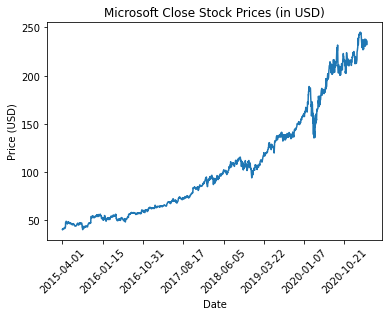
\includegraphics[width=8cm]{image/1.png}
            \caption{Microsoft (MSFT) close stock prices (in USD) over time.}
            \label{figurelabel}
        \end{figure}
        
        \textit{Analysis}: From the graph above, we can see that MSFT Stock prices experiences a general increase from 2015, with only small sudden decreases happening in 2018 and 2020. This dataset provides us with a generally increasing time series data, and we expect that our 4 models can easily pick up this forward trend and predict well in during their evaluation. 

        \subsubsection{S\&P 500 Index} The Standard \& Poor 500 Index (S\&P 500) is a stock market index tracking the performance of 500 large companies listed on stock exchanges in the United States\footnote{Wikipedia}, and the dataset that we have contains index from 1871-01-01 to 2018-04-01. Here we graph the values of the S\&P 500 Index over time in Fig. 2:

        \begin{figure}[thpb]
            \centering
            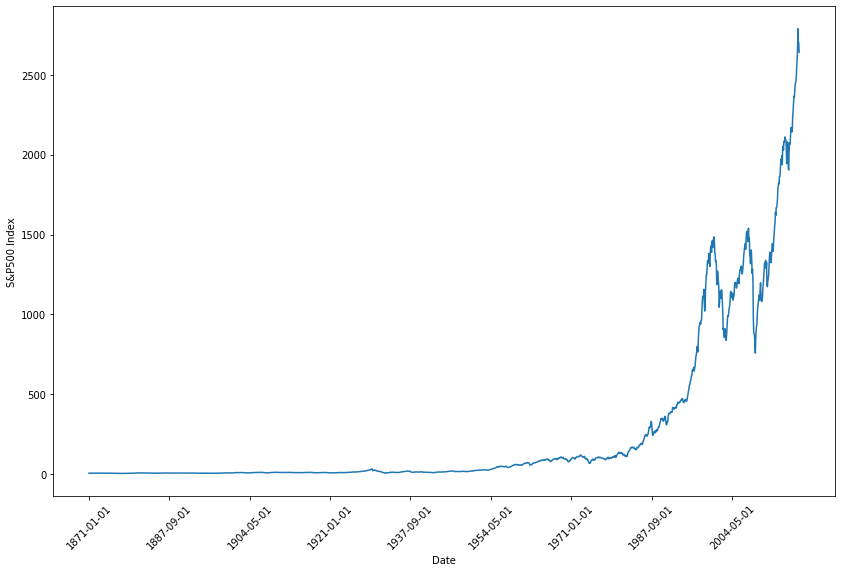
\includegraphics[width=8cm]{image/2.png}
            \caption{S\&P 500 Index over time.}
            \label{figurelabel}
        \end{figure}

        \textit{Analysis}: The reason we chose this dataset is due to its special feature: it plateaus for quite a while from 1871 to 1987, before sharply increasing and decreasing over the next 40 years, and increasing rapidly when closer to the current present. This feature is considerably different from what we observe in the MSFT stock price, where it is a general increase with small fluctuations, giving us another perspective to weigh in in our comparison.

        \subsubsection{Europe Crude Oil Prices} The dataset contains the crude oil prices (in USD) of Europe from 2015-11-02 to 2021-11-01. Here we graph the values of the Europe crude oil prices over time in Fig. 3:

        \begin{figure}[thpb]
            \centering
             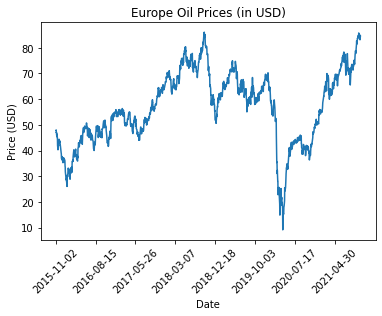
\includegraphics[width=8cm]{image/3.png}
            \caption{Europe crude oil prices (in USD) over time.}
            \label{figurelabel}
        \end{figure}

        \textit{Analysis}: This dataset contains an even more different trend than the previous two, with a high degree of fluctuation with one period of sharp increase and one period of sharp decrease back-to-back, mixed with many fluctuating plateaus also. There are no general upward or downward trends to conclude definitively. With this high entropy, we expect the 4 methods to struggle quite a bit picking up trends in these datasets. 

        \subsubsection{Bitcoin Prices} The main dataset from Kaggle offer prices of many different cryptocurrency; however, we decided to go with Bitcoin since it seems to be the most popular one currently as of 2021. The dataset contains Bitcoin prices (in USD) at close from 2013-04-29 to 2021-07-06. Here we graph the values of the Bitcoin prices at close over time in Fig. 4:

        \begin{figure}[thpb]
            \centering
              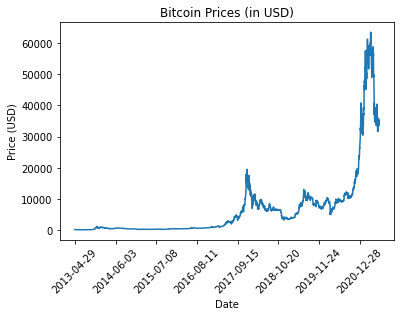
\includegraphics[width=8cm]{image/4.png}
            \caption{Bitcoin prices (in USD) at close over time.}
            \label{figurelabel}
        \end{figure}

        \textit{Analysis}: This dataset has a somewhat similar trend to the S\&P 500 one; however, after a period of a plateau from 2013 to late 2016, it is followed by a small sharp increase, then followed by a small fluctuating plateau, for 2 years, then spiking again before dropping sharply again, while the S\&P 500 contains two back-to-back series of spikes and decreases. We also expect the four methods to struggle on confidently picking up the trend as well, considering a quite unorthodox trend growth.

        \subsubsection{Artificial Data} Besides the real-life datasets listed above, we have also created an algorithm that generated artificial time series dataset, and would apply our neural networks on two which will be created during the course of our final project. The following figures showcase the trend lines of the two artificial datasets that were generated by our methods.
        \begin{figure}[thpb]
            \centering
            \includegraphics[width=7cm]{image/7.png}
            \caption{Generated time series dataset 1.}
            \label{figurelabel}
            \centering
            \includegraphics[width=7cm]{image/8.png}
            \caption{Generated time series dataset 2.}
            \label{figurelabel}
        \end{figure}

        \textit{Algorithm}: To generate an artificial time-series dataset, we first used the Pandas package to create a dataframe ranging from 2000-01-01 to 2021-12-31,  and random numbers generated by Numpy were assigned to the dataframe. Then, the seasonal decomposition method from statsmodels package was applied to the dataframe with a period of 365 days, resulting in trend, seasonality, and residual. The trend was calculated by moving average with a window length of 365, so the first half-year and the last half year will disappear. We extracted the trend data as our final artificial dataset since it is more similar to the normal financial time-series data. A total of 7307 timesteps was generated.

        \textit{Analysis}: With varying levels of increase and decreases in the trend line, these two artificial datasets should give us a good mix in our datasets pool and provide us another perspective to analyze our deep learning methods.
    
\section{Results}
    This sections details the result we received from the performance of each of the network and their corresponding analysis.
    \begin{table*}[t]
        \centering
        \captionsetup{justification=centering,margin=2cm}
        \caption{Table containing the final loss (MSE and L1) of testing and training after 50 epochs for RNN.}
        \scalebox{1.25}{
            \begin{tabular}{lllll}
                \hline
                            Dataset	&          MSE &   	&           L1 & 		\\
                \hline
                                    &     Training &      Testing &     Training &    Testing \\
                \hline
                Artificial Dataset 1 &  0.000360 &  0.001120 &    0.019259 &  0.035910 \\
                Artificial Dataset 2 &  0.000724 &   0.004046 &     0.022041 &  0.104709 \\
                Microsoft stock price &   0.000244 &  0.007969 &   0.013670 &  0.166426 \\
                    Crude oil price &   0.007576 &   0.006365 &    0.108704 &  0.126522 \\
                        S\&P 500 Index &  2.983376e-05 &   0.203713 &  0.007590 &  0.314213\\
                        Bitcoin price &  0.000479 &  0.004013 &    0.013270 &  0.153183 \\
                \hline
            \end{tabular}
        }

    \end{table*}
    \begin{table*}[t]
        \centering
        \captionsetup{justification=centering,margin=2cm}
        \caption{Table containing the final loss (MSE and L1) of testing and training after 50 epochs for BRNN.}
        \scalebox{1.25}{
            \begin{tabular}{lllll}
                \hline
                Dataset	&          MSE &   	&           L1 & 		\\
                \hline
                                    &     Training &      Testing &     Training &    Testing \\
                Artificial Dataset 1 &  0.001596 &  0.0013673 &    0.0208957 &  0.035822 \\
                Artificial Dataset 2 &  0.00019866 &   0.0030743 &     0.035325 &  0.0331284 \\
                Microsoft stock price &   0.00019866 &  0.0008362 &   0.00740934 &  0.0540353 \\
                    Crude oil price &   0.00120862 &    0.00812 &    0.02531 &  0.143351 \\
                        S\&P 500 Index &  6.157614e-06 &   0.038199 &  0.010366 &  0.56455 \\
                        Bitcoin price &  2.01082e-05 &  0.00068188 &    0.006529 &  0.0896484 \\
                \hline
            \end{tabular}
        }
    \end{table*}
    \begin{table*}[t]
        \centering
        \captionsetup{justification=centering,margin=2cm}
        \caption{Table containing the final loss (MSE and L1) of testing and training after 50 epochs for GRU.}
        \scalebox{1.25}{
            \begin{tabular}{lllll}
                \hline
                Dataset	&          MSE &   	&           L1 & 		\\
                \hline
                                    &     Training &      Testing &     Training &    Testing \\
                Artificial Dataset 1 &  0.000216833 &  0.000583076 &    0.0128767 &  0.0248689 \\
                Artificial Dataset 2 &  0.000331672 &   0.00137562 &     0.018968 &  0.0331632 \\
                Microsoft stock price &   6.8883e-05 &  0.000152029 &   0.00705973 &  0.0353123 \\
                    Crude oil price &   0.00153052 &   0.00845555 &    0.0336569 &  0.0832669 \\
                        S\&P 500 Index &  2.34019e-06 &   0.00206164 &  0.000699983 &  0.0473527 \\
                        Bitcoin price &  5.62361e-05 &  4.66154e-06 &    0.0110317 &  0.0700018 \\
                \hline
            \end{tabular}
        }
    \end{table*}
    \begin{table*}[t]
        \centering
        \captionsetup{justification=centering,margin=2cm}
        \caption{Table containing the final loss (MSE and L1) of testing and training after 50 epochs for LSTM.}
        \scalebox{1.25}{
            \begin{tabular}{lllll}
                \hline
                Dataset	&          MSE &   	&           L1 & 		\\
                \hline
                                    &     Training &      Testing &     Training &    Testing \\
                Artificial Dataset 1 &  0.00060739 &  0.00010624 &    0.01689459 &  0.005836 \\
                Artificial Dataset 2 &  0.000529 &   0.0018777 &     0.01656156 &  0.0312243 \\
                Microsoft stock price &   6.46373e-05 &  0.0015584 &   0.00786242 &  0.025047 \\
                    Crude oil price &   0.0031855 &   0.0124008 &    0.062267 &  0.127096 \\
                        S\&P 500 Index &  5.22111e-05 &   0.158363 &    0.0087754 &  0.059322 \\
                        Bitcoin price &  0.00017662 &   0.430384 &  0.00356 &  0.066288  \\
                \hline
            \end{tabular}
        }
    \end{table*}

    \subsection{Traditional RNN}
        According to the table shown below, backpropagation using the MSE loss function generally has better performance than using the L1 loss function. This phenomenon can be explained by the fact that MSE loss is based on the probabilistic assumption of a Gaussian distribution and that financial data is approximately following a normal distribution. 
    
        Since the nature of the RNN model is drawing insights from the data itself by mathematical calculations, as expected, our model can well predict the two artificial datasets, with total testing MSE loss of 0.00112 and 0.00405 respectively. As shown in the graph below, the prediction and the actual data lines almost always overlap each other.
 
        \begin{figure}[thpb]
            \centering
             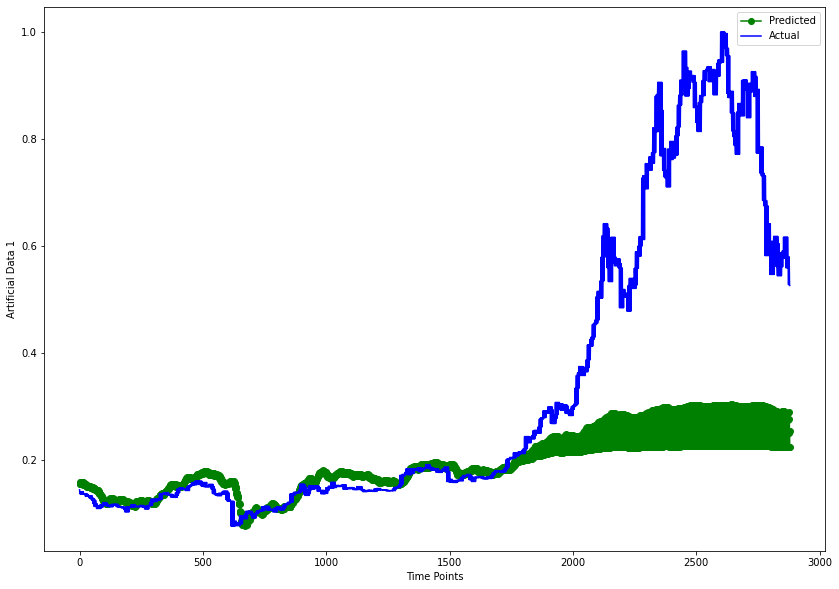
\includegraphics[width=8cm]{image/RNN/adata1_graph.png}
            \caption{Predicted values versus actual by RNN on artificial dataset 1.}
            \label{figurelabel}
        \end{figure}

        The implementation of the four real financial data is also successful with the total testing MSE loss ranging from 0.00401 to 0.204 across different datasets. The total testing MSE loss of the S\&P 500 dataset is the largest. According to the prediction and actuals comparison graph, we can see that our model can catch the general trend as well as the fluctuations of the dataset, but it keeps underestimating the values as shown in the gap between the two lines. Similar issues also appear in other financial datasets: for example, the crude oil price prediction overestimates the trough values while underestimates the peak values, and the bitcoin price prediction underestimates the peak values at the time steps 400-600. The failure may be because financial data is not perfectly normal but a normal-like distribution with fat tails, which means the real-life financial data will have more extreme values than mathematical tools predict based on probabilities. Looking at the original S\&P 500 price graph, the market demonstrates a relatively constant state from 1871 to 1971, while it dramatically increases after that. It would be difficult for the model to predict the extreme increase based on the relatively stable historical trend. 


    \subsection{Bidirectional RNN}

        As expected, bidirectional RNN performs quite better than the traditional RNN, at least with real-world datasets. While the final MSE and L1 loss of BRNN detailed above for Artificial Dataset 1 and 2 are close and some may be a bit higher than that of RNN, the performance of BRNN is much better in the real datasets. BRNN performs significantly better than RNN at predicting Microsoft stock prices and Bitcoin price, with the testing MSE loss of BRNN in predicting Bitcoin prices at 0.00068188, almost 5 times smaller than that of RNN, at 0.004013. However, it should be noted that the performance of BRNN and RNN are quite identical in the crude oil prices, with the testing MSE Loss in predicting oil prices of BRNN at 0.00812 being a bit higher than that of RNN, at 0.006365.

        \begin{figure}[thpb]
            \centering
            \includegraphics[width=8cm]{image/9.png}
            \caption{S\&P 500 Index over time. Note the long plateau period within the green box then two series of spikes in the red box.}
            \label{figurelabel}
        \end{figure}

        From observing the predicted values versus the actual graph of the S\&P 500 Index for BRNN, we observe equally bad results as that predicted by RNN. The predicted trend line seems to be overestimating decreasing and increasing compared to the actual trend lines, as seen from Fig. 11. As observed, whenever there is a slight decrease or increase in the actual trend, BRNN seems to be sharply making the turn, as seen in the 75th, 150th, 250th, and 325th-time points. Despite the loss converging and the low final testing MSE loss (0.038199), the results for S\&P 500 in observation are quite unsatisfying. This might be because of the nature of the S\&P 500's trend: there is a very long period of the plateau before sharply increasing and decreasing, which BRNN interprets that whenever there is an increase, it should do so sharply. What is surprising to us is that BRNN works well with the Bitcoin prices data, even though the trend line of Bitcoin is very similar to that of the S\&P 500's, with a period of plateau followed by a series of sharp spikes (see graph)
        
        \begin{figure}[thpb]
            \centering
            \includegraphics[width=8cm]{image/10.png}
            \caption{Bitcoin pricesover time. Note the long plateau period within the green box then two series of spikes in the red box. We can see that there are alternate between plateau or slight fluctuation and spikes, which make the bidirectional RNN pick up the trend easier compared to the S\&P500 Index trend.}
            \label{figurelabel}
        \end{figure}

        Taking a closer look, the reason why BRNN predicts better at Bitcoin despite trend similarity to S\&P 500, is because there is a moderate period between the two spikes in the Bitcoin, while the spikes in S\&P 500 happen back-to-back, which BRNN was able to smooth out its increase and decreases from.

    \subsection{GRU}

        For the two artificial datasets, GRU achieved an MSE loss of around 0.0003 on the training set and below 0.01 on the testing set; also achieved an L1 loss around 0.01 on the training set and around 0.03 on the testing set. The two loss functions for both datasets converged within 5 epochs and GRU perfectly caught all the trends and peaks. MSE loss also converged within 5 epochs for the Microsoft stock price dataset; the losses for the training set and testing set are below 0.001. There was some fluctuation for L1 loss, but ultimately it achieved 0.007 for the training dataset and 0.035 for the testing set. The prediction showed some degree of delay especially when it came to the second half of the series. GRU outperformed on the S\&P 500 Index dataset with an MSE loss of near to zero on the training set and 0.002 on the testing set, and the L1 loss confirmed the performance. The prediction did not show any delay and caught every trend and peak (Fig. 13), which is very impressive.

        \begin{figure}[h]
            \centering
            \includegraphics[width=8cm]{image/GRU/bitcoin_graph.png}
            \caption{Predicted values versus actual by GRU on Bitcoin.}
            \label{figurelabel}
        \end{figure}
        
        For the crude oil price dataset, some deviation appeared at the beginning and the end of the series with MSE loss and L1 loss below 0.1. Although both loss functions converged within 10 epochs for the Bitcoin price dataset, using the MSE loss function for backpropagation resulted in a lower loss on both the training set and testing set. It also successfully predicted the extreme peak at the end of the series.

    \subsection{LSTM}

        The LSTM model is expected to perform best compared with the other models in theory as it could use both information from the long and short term when outputting the prediction. Throughout the testing with datasets, we could see the usual common thing is that both test and train loss decrease over time which signals that our model for LSTM is not in overfitting issue. But for the cases when having datasets with extreme increases suddenly in their values, the model fails to capture that successfully. On the other hand, the LSTM seems to do very well on the artificial dataset and the ones that don’t have a sudden big changes in their values throughout time. It could just capture the shape slightly but not to what we expect. The train and test overall have some volatile shape in their plots at some points before the convergence.

        \begin{table*}[th] \centering
            \captionsetup{justification=centering,margin=2cm}
            \caption{Final testing MSE loss comparison table\\ (highlighted means lowest loss of four networks in corresponding dataset)}
            \begin{threeparttable}
                \scalebox{1.25}{
                    \begin{tabular}{l|ll|llll}
                        \hline
                        Neural Network & A. Data 1 & A. Data 2 & Microsoft & S\&P 500 & Crude oil & Bitcoin\\
                        \hline
                        RNN &   0.001120 &      0.004046 & 0.007969 & 0.006365 & 0.203713 & 0.004013\\
                        BRNN & 0.0013673 &     0.0030743 & 0.0008362 & \textbf{0.00812} & 0.038199 & 0.00068188\\
                        GRU &               0.000583076 &   \textbf{0.00137562} & \textbf{0.000152029} & 0.00845555 & \textbf{0.00206164} & \textbf{4.66154e-06}\\
                        LSTM &              \textbf{0.00010624} &    0.0018777 & 0.0015584 & 0.0124008 & 0.158363 & 0.430384\\
                        \hline
                    \end{tabular}
                }
            \end{threeparttable}
        \end{table*}
        \begin{table*}[th] \centering
            \captionsetup{justification=centering,margin=2cm}
            \caption{Final testing L1 loss comparison table\\ (highlighted means lowest loss of four networks in corresponding dataset)}
            \begin{threeparttable}
                \scalebox{1.25}{
                    \begin{tabular}{l|ll|llll}
                        \hline
                        Neural Network & A. Data 1 & A. Data 2 & Microsoft & S\&P 500 & Crude oil & Bitcoin\\
                        \hline
                        RNN &   0.035910 &      0.104709 & 0.166426 & 0.126522 & 0.314213 & 0.153183\\
                        BRNN & 0.035822 &      0.0331284 & 0.0540353 & 0.143351 & 0.56455 & 0.0896484\\
                        GRU &               0.0248689 &   0.0331632 & 0.0353123 & \textbf{0.0832669} & \textbf{0.0473527} & 0.0700018\\
                        LSTM &              \textbf{0.005836} &    \textbf{0.0312243} & \textbf{0.025047} & 0.127096 & 0.059322 & \textbf{0.066288}\\
                        \hline
                    \end{tabular}
                }
            \end{threeparttable}
        \end{table*}

        \begin{figure*}
            \centering
            \begin{minipage}{\columnwidth}
                \centering
                \includegraphics[width=8cm]{image/GRU/bitcoin_graph.png}
                \subcaption{Prediction by GRU, for Bitcoin prices}
                \label{label1}
            \end{minipage}%
            \begin{minipage}{\columnwidth}
                \centering
                \includegraphics[width=8cm]{image/LSTM/bitcoin_graph.png}
                \subcaption{Prediction by LSTM, for Bitcoin prices}
                \label{label2}
            \end{minipage}
            \begin{minipage}{\columnwidth}
                \centering
                \includegraphics[width=8cm]{image/GRU/sp500_graph.png}
                \subcaption{Prediction by GRU, for S\&P 500 Index}
                \label{label3}
            \end{minipage}%
            \begin{minipage}{\columnwidth}
                \centering
                \includegraphics[width=8cm]{image/LSTM/sp500_graph.png}
                \subcaption{Prediction by LSTM, for S\&P 500 Index}
                \label{label4}
            \end{minipage}
            \captionsetup{margin=1.5cm}
            \caption{Graphs showing the predicted values versus actual for a certain part of the corresponding dataset. Note the extreme difference in performance between GRU and LSTM in the Bitcoin prices and the S\&P 500 index dataset. Even though LSTM and GRU possess similar losses in the L1 metric, GRU appears to have a more accurate prediction than LSTM, when observed in the above graphs.}
        \end{figure*}
    \subsection{Overall analysis}
        Table VI and VII show the final testing MSE and L1 loss, respectively, in all 6 datasets among the four analyzed networks. Of the four networks, LSTM seems to be the best performing, having the lowest loss in both MSE and L1 in artificial dataset 1, and the lowest loss in artificial dataset 2 in L1 loss, though just slightly lower than that of bidirectional RNN and GRU, about 0.02 difference. In general, all four networks' loss seem to be converging over the course of the training process, so we can conclude that these methods all work well with artificial data.

        Regarding actual datasets, GRU seems to have the performance when it comes to using MSE loss for the actual datsets, with 3 out of 4 real-world datasets having the lowest loss out of the 4 network, with its final testing loss in S\&P 500 at 0.0084555 being very close to the one with the lowest loss, which is BRNN at 0.00812. We are confident that if we run the implementation again GRU will be able to perform better than BRNN. With regard to L1 loss, it seems that LSTM perform equally well to GRU, having the lowest loss in 2 out the four real-world datasets. Both networks' loss seem to have only slight difference from each other (see above tables), so we can say that based on L1 loss there are no definitive best networks for these 4 datasets. However, when observing the predictions versus actual values graph for GRU and LSTM, it seems that GRU has a more accurate predictions than LSTM (see Fig. 9). This is quite an interesting observation, considering the extereme difference in actual performance when there are similarity in L1 losses for GRU and LSTM. We are not sure why this happened, and would like to investigate the cause for this, but due to time constraint we will leave this at that.
        
        Overall, when considered the final testing losses of both MSE and L1 for all 6 applied datasets of the 4 models, overall GRU was effectively applied to financial time-series data and had the best performance on all datasets compared to other models.

\section{Dicussion}
    \subsection{What to say about our result}
        Since there are already many research papers written for this exact same subject, that is, deep learning in time series, our project serves to only reinforce and certify some claims put forward by some of our predecessors. As we have noted before, this is not a novel approach to time series analysis. However, we still went ahead with this project idea anyway, since it might help to confirm others' conclusion in this field of deep learning.

    \subsection{Shortcomings}
        This project was not completed without any shortcomings, and so we would like to discuss some that could improve our overall analysis. The first thing is that since the four models were individually developed by each of the person in our team, we might have a synchronization problem: the implementation (the overall model structure and the boilerplate training code) we wrote was not centralized until the very end of the project period, so there might exist some bias between a model might perform better than the others not due to its nature, but due to the actual code that was written for it. This is a potentially serious problem that could affect our overall analysis.

        Another shortcoming is the one that has been mentioned above: there are some non-deterministic discrepancies between the final testing L1 loss of GRU and LSTM and the predictions they produce. If given more time, we could have probed more at our implementation and understand the cause, but for now we will leave it at this.  
        

\section{Conclusion}
    By taking a look at four recurrent neural network structures and using them for prediction in both real-life and artificial financial datasets, we were able to analyze the performance of deep learning in price prediction. Overall, the four models we chose, traditional RNN, bidirectional RNN, GRU, and LSTM, peform well with this task of time series analysis, as observed from their converging losses on the 6 datasets, 4 real-world, 2 artificial. Of the four models that we experiemented with, GRU performs the best, despite our initial expectation that LSTM would be the one with the better performance. There are some issues that we have mentioned in the shortcomings section above, but in general, we believe our analysis is quite satisfactory for this project. It was interesting to see how deep learning models were able to be trained into predicting time series data, with a good performance. If possible, we would like to compare the performance of deep learning with that of the autoregressive methods, which we believe will give us some interesting results and insights.


\section{Division of Labor}
    The work of this project was split evenly between the team members. We will be elaborating the division of labor in each stage of this final project by providing a table of who did what in the following sections:

    \subsection{Prospectus}
        We first need to analyze our datasets to pull out statistics and some general trends. The table below shows who is responsible for the dataset analysis

            % Team member(s) & Dataset\\
            % Quianwen and Chuqin & Microsoft stock prices and S&P 500 Index\\
            % Vuong and Minh Khoi & Crude oil prices and Bitcoin prices
    
        The team member responsible for compiling information and writing the prospectus was Vuong.

    \subsection{Presentation}
        \subsubsection{Neural network implementation} We have split up the four neural networks implementation responsiblity as detailed in the following table:
            \begin{table}[h!] \centering
                \caption{Datasets}
                \begin{threeparttable}
                    \begin{tabular}{|c|c|}
                        \hline
                        Neural Network Name & Implementer\\
                        \hline
                        Traditional RNN & Qianwen\\
                        Bidirectional RNN & Vuong\\
                        GRU & Chuqin\\
                        LSTM & Minh Khoi\\
                        \hline
                    \end{tabular}
                \end{threeparttable}
            \end{table}

        Each person was also responsible for applying their implementation to the datasets, as well as conducting analysis on the results. With their results, each person went ahead and write up their own report and analysis, which was be pieced together in the presentation.

        The presentation was compiled from the four report and graphs of each team members, and all four members contributed to the slides, whether content or design.

    \subsection{Final report}
        Similar to the presentation, each team member was responsible for their own report of their assigned neural network. The final report was put together in LaTeX by Vuong.

\section{Appendix}
    In this section we put the predicted values versus actual along with loss behavior graphs for our analysis. This can be used for reference.

\cite{PURUSHOTHAM2018112}

\bibliographystyle{unsrt}
\bibliography{reference}

\end{document}
